% 02_preliminaries.tex
%
% Purpose:
%   Collect geometry, quasiperiodicity, the scalar transmission model, Rayleigh
%   trace coordinates, and the two global workflows before the main
%   trace-subspace formulation.
%
% Main algorithm:
%   This section defines the variables, function spaces, and matrix problem
%   types used later.  It does not introduce the lead-cell Bloch algorithm.
%
% Based on:
%   sections/intro.tex, sections/problem.tex, and sections/trace_spaces.tex from
%   the first report draft.
%
% Main changes:
%   Moves geometry and Rayleigh coordinates out of separate top-level sections
%   and places them under a standard preliminaries section.
%
% Numerical goal:
%   Fix the notation used by the matrix assembly and validation workflow.

\section{Preliminaries}

\subsection{Geometry and quasiperiodicity}

The longitudinal lead direction is \(x\).  The transverse quasiperiodic
direction is \(y\), with period \(d\).  The field satisfies
\[
  u(x,y+d)=\ee^{\ii\beta d}u(x,y),
\]
where \(\beta\) is the transverse quasimomentum.  The three reference cells
nearest the defect are
\[
  \Ccell^-,
  \qquad
  \Ccell^0,
  \qquad
  \Ccell^+ .
\]
The center obstacle is \(\Omega_0\), with boundary
\[
  \Sigma=\partial\Omega_0 .
\]
The adjacent lead obstacles are denoted \(\Omega_-\) and \(\Omega_+\).  The
artificial center-cell ports are
\[
  \Gamma_-=\{x=X_-\},
  \qquad
  \Gamma_+=\{x=X_+\}.
\]
Their outward normals, always taken with respect to the center cell, are
\[
  \nu_{\Gamma_-}=-e_x,
  \qquad
  \nu_{\Gamma_+}=+e_x .
\]
When the longitudinal periods of the two half-leads are needed, they are written
\(L_-\) and \(L_+\).  The symbol \(d\) is reserved for the transverse
quasiperiodic period.

\begin{figure}[ht]
\centering
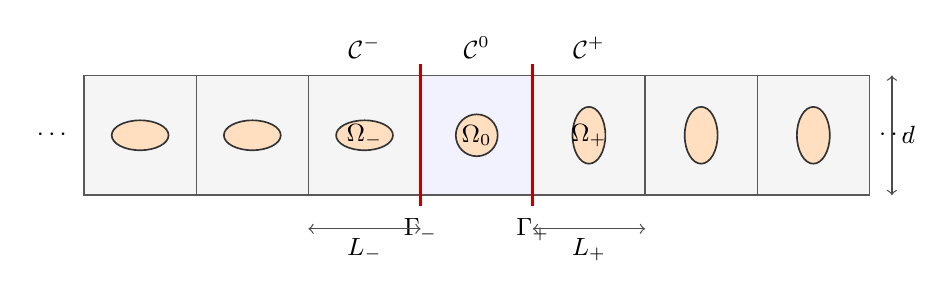
\begin{tikzpicture}[
  x=0.95cm,
  y=0.95cm,
  every node/.style={font=\small},
  cell/.style={draw=black!65, line width=0.5pt},
  leadcell/.style={fill=gray!8},
  centercell/.style={fill=blue!5},
  inclusion/.style={draw=black!80, fill=orange!25, line width=0.6pt},
  port/.style={draw=red!75!black, line width=1.1pt},
  dim/.style={<->, draw=black!70, line width=0.45pt}
]
  \foreach \x in {-5.25,-3.75,-2.25} {
    \draw[cell, leadcell] (\x,-0.8) rectangle ++(1.5,1.6);
    \draw[inclusion] (\x+0.75,0) ellipse [x radius=0.38, y radius=0.20];
  }

  \draw[cell, centercell] (-0.75,-0.8) rectangle (0.75,0.8);
  \draw[inclusion] (0,0) circle [radius=0.28];

  \foreach \x in {0.75,2.25,3.75} {
    \draw[cell, leadcell] (\x,-0.8) rectangle ++(1.5,1.6);
    \draw[inclusion] (\x+0.75,0) ellipse [x radius=0.22, y radius=0.38];
  }

  \draw[port] (-0.75,-0.95) -- (-0.75,0.95);
  \draw[port] (0.75,-0.95) -- (0.75,0.95);

  \node[above] at (-1.5,0.9) {$\mathcal C^-$};
  \node[above] at (0,0.9) {$\mathcal C^0$};
  \node[above] at (1.5,0.9) {$\mathcal C^+$};

  \node[below] at (-0.75,-0.98) {$\Gamma_-$};
  \node[below] at (0.75,-0.98) {$\Gamma_+$};

  \node at (-1.5,0) {$\Omega_-$};
  \node at (0,0) {$\Omega_0$};
  \node at (1.5,0) {$\Omega_+$};

  \draw[dim] (-2.25,-1.25) -- (-0.75,-1.25);
  \node[below] at (-1.5,-1.25) {$L_-$};
  \draw[dim] (0.75,-1.25) -- (2.25,-1.25);
  \node[below] at (1.5,-1.25) {$L_+$};

  \draw[dim] (5.55,-0.8) -- (5.55,0.8);
  \node[right] at (5.55,0) {$d$};
  \node[left] at (-5.35,0) {$\cdots$};
  \node[right] at (5.25,0) {$\cdots$};
\end{tikzpicture}
\caption{Schematic of the center cell, adjacent periodic lead cells, and compact
ports.  The diagram is not a geometry specification; the actual inclusion shapes
are supplied by the geometry routines.}
\label{fig:cells}
\end{figure}

\subsection{Helmholtz transmission problem}

In each homogeneous material region the field satisfies a scalar Helmholtz
equation.  In the exterior background and inside an inclusion we write
\[
  (\Delta+k_e^2)u_e=0,
  \qquad
  (\Delta+k_i^2)u_i=0 .
\]
For a dielectric inclusion with relative index \(n\), one often has
\(k_i=nk_e\), but the formulation only uses the exterior and interior
wavenumbers supplied to the boundary integral assembly.

Across a smooth material interface \(\Sigma_j=\partial\Omega_j\), the TM-like
transmission conditions used in the current formulation are
\[
  u_e=u_i,
  \qquad
  \partial_\nu u_e=\partial_\nu u_i .
\]
Here \(\nu\) is the unit normal pointing out of the inclusion.  A TE variant
would replace the Neumann continuity by a weighted normal derivative condition,
but that is a change in the boundary condition row rather than in the
trace-subspace idea.

\subsection{Rayleigh trace coordinates}

On a vertical port \(x=X\), the transverse quasiperiodicity suggests the
Rayleigh basis
\[
  \beta_m=\beta+\frac{2\pi m}{d},
  \qquad
  \psi_m(y)=\frac{1}{\sqrt d}\ee^{\ii\beta_m y},
  \qquad
  m\in\mathbb Z .
\]
The longitudinal Rayleigh wavenumber is
\[
  \gamma_m=\sqrt{k^2-\beta_m^2},
  \qquad
  \operatorname{Im}\gamma_m\ge 0 .
\]
After truncation to \(|m|\le M\),
\[
  K=2M+1 .
\]
For each port \(\Gamma_\pm\), the Dirichlet and outward-normal derivative trace
coefficients are
\[
  D^\pm\in\CC^K,
  \qquad
  N^\pm\in\CC^K .
\]
At the continuous level, the corresponding Cauchy trace space is
\[
  H^{1/2}(\Gamma_\pm)\times H^{-1/2}(\Gamma_\pm).
\]
After truncation, the ambient coordinate space is
\[
  \Tspace_M=\CC_D^K\times\CC_N^K .
\]
This is only an ambient coordinate space.  Physical incoming and outgoing traces
will be selected as subspaces of \(\Tspace_M\) by the periodic half-lead
calculation.

\subsection{Scattering and eigenvalue workflows}

In a forced scattering problem, the data are incoming Bloch traces from one or
both half-leads, and the scattered part is required to be outgoing or admissible
in each half-lead.  The discretized system has the form
\[
  \Atr(k,\beta)x=b_{\mathrm{in}} .
\]
The right-hand side is not an arbitrary wall trace; it must belong to the
incoming trace subspace:
\[
  \begin{bmatrix}
  D_{\mathrm{in,tot}}^\pm\\
  N_{\mathrm{in,tot}}^\pm
  \end{bmatrix}
  =
  \begin{bmatrix}
  \Din^\pm\\
  \Nin^\pm
  \end{bmatrix}p_{\mathrm{in}}^\pm .
\]

For a defect-mode or transmission-eigenvalue-type calculation, the same matrix
is used without forcing:
\[
  \Atr(k,\beta)x=0 .
\]
Numerically, one scans for parameter values where
\[
  \sigmin(\Atr(k,\beta))\approx 0 .
\]
Thus the same assembly supports both well-posed forced solves away from
resonances and homogeneous searches for nontrivial admissible null vectors.
